\documentclass{beamer}

\usepackage{graphicx}
\usepackage{booktabs}\title[Chiselizing SDR Blocks]{Chiselizing SDR Blocks}
\author{Albert Magyar}
\date{\today}

\begin{document}
\begin{frame}
\titlepage
\end{frame}

\begin{frame}
\frametitle{Overview}
\begin{itemize}
\item Intro to RFNoC
\item RFNoC Blocks
\item Example: \texttt{addsub}
\item Recurring patterns in Verilog and Chisel
\item Goals
\end{itemize}
\end{frame}

\begin{frame}
\frametitle{Intro to RFNoC}
\begin{center}
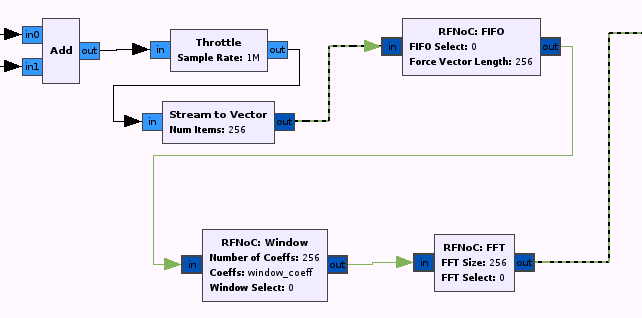
\includegraphics[width=3.5in]{images/gnu_radio_rfnoc.png}
\end{center}
\begin{itemize}
\item FPGA toolkit for GNU radio
\item Allows chaining of hardware and software blocks 
\end{itemize}
\end{frame}

\begin{frame}
\frametitle{Intro to RFNoC}
\begin{itemize}
\item Accelerators implemented in Verilog
\item NoC: packet headers on top of AXI4 Streaming crossbar
\item Designers write parametrized blocks with ready/valid/last and settings registers
\end{itemize}
\end{frame}

\begin{frame}
\frametitle{Intro to RFNoC}
\begin{itemize}
\item Designers write parametrized blocks
\item GNU Radio frontend elaborates instances
\item RFNoC configurator assigns endpoint addresses and parametrizes RFNoC shim modules (\texttt{noc\_shell}) 
\item Parametrizes and generates Verilog for NoC
\end{itemize}
\end{frame}

\begin{frame}
\frametitle{RFNoC Blocks}
\begin{itemize}
\item Simple, fixed-function DSP blocks
\item Blocks have simple FIFO interfaces
\item Export parameters to the GNU Radio space
\item Identity as RFNoC endpoint transparent to designer
\item<2-> \emph{We want people to write these in Chisel}
\end{itemize}
\end{frame}


\end{document}